% !TeX spellcheck = de_DE
% !TeX root = kristallographie_skript.tex
\begin{definition}
Eine \udot{starre Bewegung} oder \udot{Isometrie} ist eine Abbildung $\phi:\IR^n\to\IR^n$, die abstandserhaltend ist, d.h.
\[\forall x,y\in\IR^n: \norm{\phi(x)-\phi(y)} = \norm{x-y}\]
\end{definition}

\begin{example}
\begin{enumerate}
\item Translationen: $\tau_v(x) := x+v$.
\item Drehungen im $\IR^3$: Bis auf Koordinatenwahl die Abbildungen der Form
\[\begin{pmatrix}x\\y\\z\end{pmatrix}\mapsto\begin{pmatrix}
\cos(\alpha)x + (-\sin(\alpha)) y \\
\sin(\alpha)x + \cos(\alpha)y \\
z
\end{pmatrix}\]
$\alpha$ wird dabei als Drehwinkel bezeichnet. Die Drehachse erkennt man daran, dass es eine Gerade $A\subseteq\IR^3$ ist, die $D(A)=A$ erfüllt. In obiger Beschreibung ist das Koordinatensystem so gewählt worden, dass die Drehachse genau die Gerade $\Set{\begin{psmallmatrix}0\\0\\z\end{psmallmatrix} | z\in\IR}$ ist.
\item Inversionen = Punktspiegelungen
\item Spiegelungen an einer Geraden (in $\IR^2$) bzw. an einer Ebene (in $\IR^3$) bzw. allgemein an einer Hyperebene ($(n-1)$-dimensionale Unterräume von $\IR^n$).
\item Wenn $f,g$ Isometrien sind, dann auch $f\circ g$, z.B.
\begin{enumerate}
\item Gleitspiegelungen: Im eine Spiegelung an einer Geraden (in $\IR^2$), einer Ebene (im $\IR^3$) bzw. allgemeiner einer Hyperebene gefolgt von einer Translation in Richtung eines Vektors parallel zu dieser Geraden / Ebene / Hyperebene.
\item Drehinversionen: Eine Drehung $g$ gefolgt von einer Inversion $f$ in einem Punkt auf der Drehachse von $g$.
\item Schraubungen: Eine Drehung $g$ gefolgt von einer Translation $f$ entlang der Drehachse.
\end{enumerate}
\item Die Identität $\id: x\mapsto x$. Das ist gleichzeitig die Translation um die Distanz $0$ (in jede Richtung) und die Drehung um den Winkel $0$ (mit jeder Drehachse).
\end{enumerate}
\end{example}

\begin{table}[htp]
	\caption{Symbolnotationen für Bewegungen ohne Translationsanteil}
	\begin{tabular}{cC{4cm}C{5cm}c}
		\toprule
		Symbol    & Hermann-Maguin-Symbol       & Symmetrien                                  & Gruppenordnung \\
		\midrule
		\sym{0}   & $\overline{1}$                             & Inversion                                   & 1              \\
		\sym{2}   & $2$                                        & 2-zählige Drehung                           & 1              \\
		\sym{3}   & $3$                                        & 3-zählige Drehung                           & 3              \\
		\sym{4}   & $4$                                        & 4-zählige Drehung                           & 4              \\
		\sym{6}   & $6$                                        & 6-zählige Drehung                           & 6              \\
		\sym{20} & $m \hspace{0.5cm}(=\overline{2})$           & Ebenenspiegelung                            & 2              \\
		\sym{30}  & $\overline{3}$ \enquote{drei quer}         & 3-zählige Drehinversion                     & 6              \\
		\sym{84}  & $\overline{4}$ \enquote{vier quer}         & 4-zählige Drehinversion                     & 4              \\
		\sym{36}  & $\overline{6}$ \enquote{sechs quer}        & 6-zählige Drehinversion                     & 6              \\
		\sym{102} & $\frac{2}{m}$ \enquote{zwei über m}        & Spiegelung \& 2-zählige Drehung um Spiegelebenennormale & 4              \\
		\sym{103} & $\frac{3}{m} = \overline{6}$ \enquote{drei über m} & Spiegelung \& 3-zählige Drehung um Spiegelebenennormale & 6 \\
		\bottomrule
\label{table:symbole_punkt}
	\end{tabular}

	\bigskip
	
	\caption{Symbolnotationen für Bewegungen mit Translationsanteil}
	\begin{tabular}{C{1.5cm}C{3cm}C{5cm}C{3cm}c}
		\toprule
		Symbol                                                       & Hermann-Maguin-Symbol       & Symmetrien mit Translation um $t$                                                                                                                                                                       & Ordnung der induzierten Punktgruppe & \\
		\midrule
		\sym{21}                                                     & $2_1$                                      & 2-zählige Schraubung, $t=\frac{1}{2}$                                                                                                                                                                       & 2                      &  \\
		\sym{31} \ \  \sym{32}                                       & $3_1$ \ \  $3_2$                           & 3-zählige Schraubung, $t=\frac{1}{3}, t=\frac{2}{3}$                                                                                                                                                       & 3                       & \\
		\sym{41}\ \  \sym{42} \ \ \sym{43}                           & $4_1$ \ \ $4_2$ \ \newline $4_3$                  & 4-zählige Schraubung, $t=\frac{1}{4}, t=\frac{2}{4}, t=\frac{3}{4}$                                                                                                                                        & 4                        & \\
		\sym{61} \ \ \sym{62} \ \ \sym{63} \ \ \sym{64} \ \ \sym{65} & $6_1 \ \ 6_2$ \ \newline $6_3$ \ \ $6_4$ \ \newline $6_5$ & 6-zählige Schraubung, $t=\frac{1}{6}, t=\frac{2}{6}, t=\frac{3}{6},$\newline$ t=\frac{4}{6}, t=\frac{5}{6}$                                                                                                          & 6                       & \\
		\sym{9}                                                      & $a, b, c, n, d$                            &  Gleitspiegelung, $t=\frac{1}{2}\vc{a}, t=\frac{1}{2}\vc{b}, t=\frac{1}{2}\vc{c}, t=\frac{1}{2}(\vc{\tau_1}+\vc{\tau_2}), t=\frac{1}{4}(\vc{\tau_1} +\vc{\tau_2}) $ & 2, 4 & \\                  
		\bottomrule
\label{table:symbole_raum}
	\end{tabular}
\end{table}

\begin{definition}
Angenommen, wir haben einen Nullpunkt gewählt. Eine Isometrie, die den Nullpunkt fixiert, wird \udot{orthogonale} Abbildung genannt.
\end{definition}

\begin{theorem}
Es sei $f:\IR^n\to\IR^n$ eine Bewegung. Dann gilt:
\begin{enumerate}
\item $f$ ist \udot{affin}, d.h.
\[\forall p_0,p_1\in\IR^n, \lambda\in\IR: f(\lambda p_1 + (1-\lambda)p_0) = \lambda f(p_1)+(1-\lambda)f(p_0)\]
\item Haben wir einen Nullpunkt gewählt und ist $f$ orthogonal, dann ist $f$ sogar \udot{linear}, d.h.
\begin{enumerate}
\item $\forall v_1,v_2\in\IR^n: f(v_1+v_2)=f(v_1)+f(v_2)$
\item $\forall v\in\IR^n, \lambda\in\IR: f(\lambda v)=\lambda f(v)$.
\end{enumerate}
\item $f$ erhält das Skalarprodukt von Vektoren und Winkel zwischen Vektoren.
\end{enumerate}
\end{theorem}
\begin{proof}
a. Sei zunächst $0\leq \lambda\leq 1$. Der Punkt $\lambda p_1+(1-\lambda)p_0 = p_0+\lambda(p_1-p_0) = p_1-(1-\lambda)(p_1-p_0)$ ist genau derjenige Punkt, der genau Abstand $\lambda\norm{p_1-p_0}$ von $p_0$ und $(1-\lambda)\norm{p_1-p_0}$ von $p_1$ hat und es gibt nur einen solchen Punkt. Daher ist $f(\lambda p_1+(1-\lambda)p_0)$ genau derjenige Punkt, der den Abstand $\lambda\norm{p_1-p_0}=\lambda\norm{f(p_1)-f(p_0)}$ von $f(p_0)$ und den Abstand $(1-\lambda)\norm{p_1-p_0} = (1-\lambda)\norm{f(p_1)-f(p_0)}$ von $f(p_1)$ hat. Weil es nur einen solchen Punkt gibt, muss $f(\lambda p_1+(1-\lambda)p_0) = \lambda f(p_0)+(1-\lambda)f(p_1)$ sein.

Im allgemeinen Fall liegen die drei Punkte $p_0$, $p_1$ und $p_\lambda:=\lambda p_1+(1-\lambda)p_0$ ja auf einer gemeinsamen Geraden. Es gibt also immer einen, der zwischen den anderen zweien positioniert ist. Wenn das z.B. $p_0$ ist, dann gibt es eine Gleichung der Form $p_0 = \alpha p_\lambda + (1-\alpha)p_1$ mit $\alpha\in [0,1]$ (Übung: Man berechne $\alpha$ aus $\lambda$ und umgekehrt). Wenn $p_1$ zwischen $p_0$ und $p_\lambda$ liegt, gibt es analog eine Gleichung der Form $p_1=\beta p_\lambda + (1-\beta)p_1$ mit $\beta\in[0,1]$. In beiden Fällen folgt aus dem schon bewiesenen auch die gleiche Gleichung für $f(p_0)$, $f(p_1)$ und $f(p_\lambda)$.

\medbreak
b. Wenn $f(0)=0$ ist, dann können wir $p_0=0$ und $p_1=v$ in a. einsetzen und erhalten direkt, dass $f(\lambda v)=\lambda f(v)$ gilt.

Daraus folgern wir nun:
\[f(v_1+v_2) = 2f(\tfrac{1}{2}(v_1+v_2)) = 2f(\tfrac{1}{2}v_1 + \tfrac{1}{2}v_2) \overset{a.}{=} 2(\tfrac{1}{2}f(v_1)+\tfrac{1}{2}f(v_2))=f(v_1)+f(v_2)\]

\medbreak
c. folgt aus $\tfrac{1}{2}(\norm{v_1+v_2}^2-\norm{v_1}^2-\norm{v_2}^2)=\braket{v_1,v_2}$, $\norm{v}=\norm{f(v)}$ und b.

Winkelerhaltung folgt dann aus $\cos(\sphericalangle(v_1,v_2)) = \frac{\braket{v_1,v_2}}{\norm{v_1}\cdot\norm{v_2}}$.
\end{proof}

\begin{remark}
Aus der Linearität und der Tatsache, dass wir nur Räume endlicher Dimension betrachten, kann man folgern, dass jede Isometrie bijektiv ist, also eine Umkehrabbildung besitzt. Die Umkehrabbildung muss dann selbst wieder eine Isometrie sein, denn:
\[\norm{p_1-p_2} = \norm{f(f^{-1}(p_1))-f(f^{-1}(p_2))} = \norm{f^{-1}(p_1)-f^{-1}(p_2)}\]
\end{remark}

\subsection{Klassifikation der Bewegungen}

\begin{lemma}[Reduktion von beliebigen auf orthogonale Bewegungen]
Haben wir einen Nullpunkt gewählt, dann ist ein beliebiges $f\in\Isom(\IR^n)$ eine orthogonale Abbildung gefolgt von einer Translation (mglw. um den Abstand $0$).
\end{lemma}
\begin{proof}
Ist $f(0)=:v$, dann betrachten wir die Translation $\tau_v$. Dann ist nämlich $(\tau_v^{-1}\circ f)(0) = 0$, also ist $f=\tau_v\circ(\tau_v^{-1}\circ f)$ eine Komposition aus der orthogonalen Abbildung $\tau_v^{-1}\circ f$ gefolgt von der Translation $\tau_v$.
\end{proof}

\begin{theorem}[Klassifikation von Bewegungen in kleinen Dimensionen]
Alle orthogonalen Abbildungen des
\begin{enumerate}
\item $\IR^1$ sind die Identität oder Spiegelung im Nullpunkt.
\item $\IR^2$ sind Drehungen (ggf. um den Winkel $0$) um den Nullpunkt oder Spiegelungen an Geraden durch den Nullpunkt.
\item $\IR^3$ sind Drehungen oder Drehinversionen (ggf. um den Drehwinkel $0$) um eine Achse durch den Nullpunkt oder Ebenenspiegelungen an Ebenen durch den Nullpunkt.
\end{enumerate}

Allgemeiner: Alle Bewegungen des
\begin{enumerate}
\item $\IR^1$ sind Translationen oder Spiegelungen.
\item $\IR^2$ sind Drehungen (ggf. um den Drehwinkel $0$) oder Geradenspiegelungen gefolgt von einer Translation (ggf. um den Abstand $0$).
\item $\IR^3$ sind Drehungen oder Drehinversionen (ggf. um den Drehwinkel $0$) oder Ebenenspiegelungen gefolgt von einer Translation (ggf. um den Abstand $0$).
\end{enumerate}
\end{theorem}

\subsection{Stereographische Projektion}
Mittels der \udot{stereographischen Projektion} werden alle Punkte auf der Kugeloberfläche von $S^2$ bis auf dem Südpol als Punkte auf einer Ebene dargestellt. Wir nutzen sie, um Orientierungen von Vektoren im dreidimensionalen Raum zueinander im zweidimensionalen Raum darzustellen. Diese Vektoren können verschiedenes symbolisieren, bei uns meist die Orientierung von Drehachsen und Flächennormalen von konvexen Körpern.
\begin{figure}%{0.5\linewidth}
\centering
\begin{subfigure}{0.4\textwidth}
	\centering
	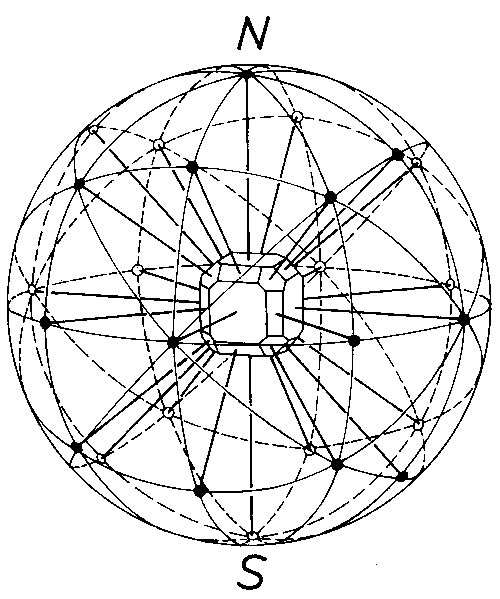
\includegraphics[width=0.8\linewidth]{./pictures/stpr1.jpg}
	\caption{Schnittpunkte der Flächennormalen auf $S^2$}
\end{subfigure}%
\begin{subfigure}{0.4\textwidth}
	\centering
	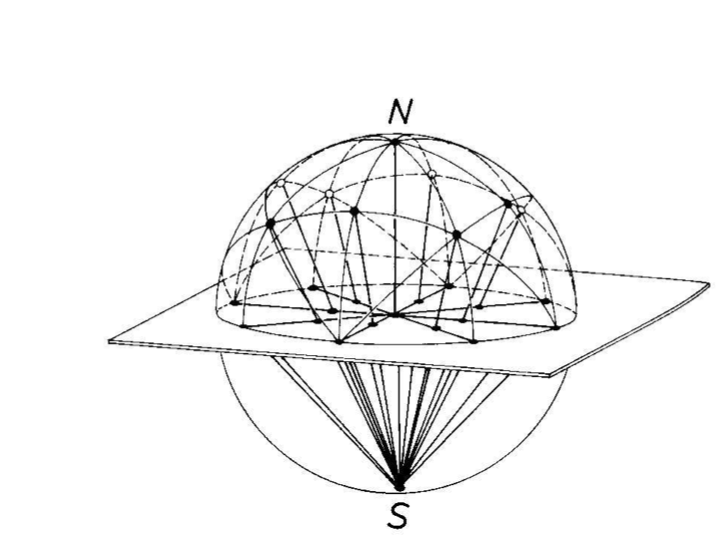
\includegraphics[width=1.2\linewidth]{./pictures/stpr2.jpg}
	\caption{Projektion auf die Äquatorebene}
\end{subfigure}
\caption{Stereographische Projektion eines konvexen Körpers}
\end{figure}

\begin{figure}
	\centering
	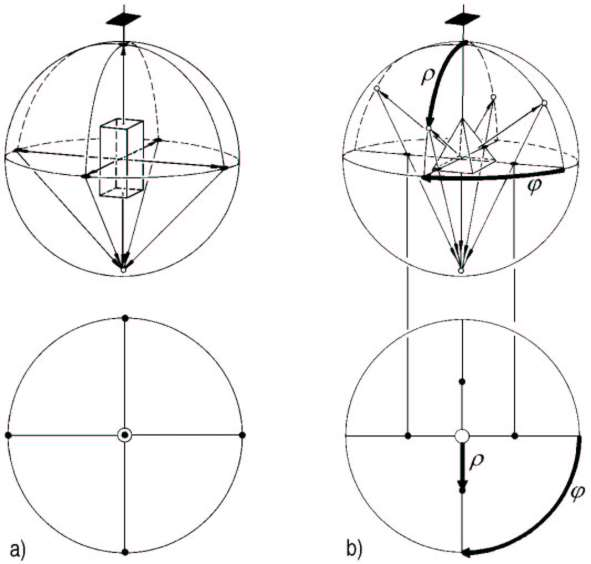
\includegraphics[width=0.8\linewidth]{./pictures/stpr3.jpg}
	\caption{Stereographische Projektion verschiedener Körper}
\end{figure}

\begin{figure}
	\centering
\begin{subfigure}{1\textwidth}
	\centering
	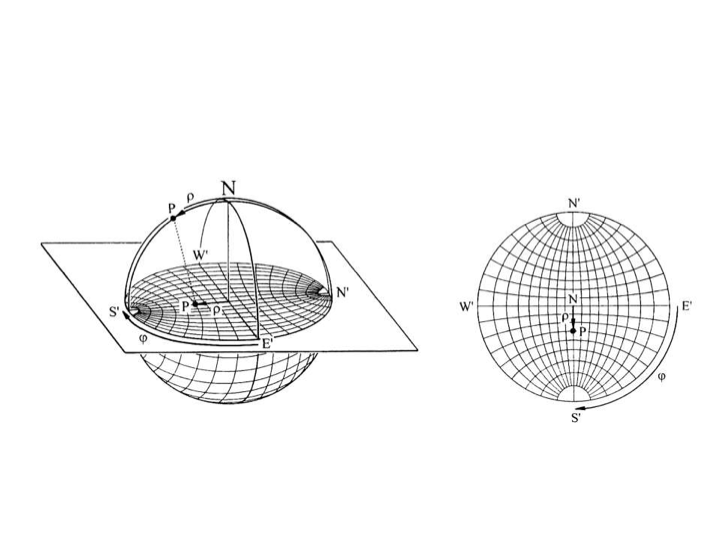
\includegraphics[width=1.1\linewidth]{./pictures/stpr4.jpg}
	\caption{Lage der Winkel $\phi$ und $\rho$}
\end{subfigure}
\begin{subfigure}{0.9\textwidth}
	\centering
	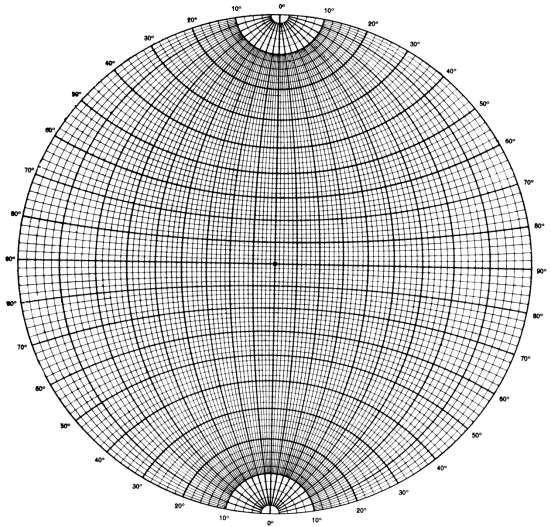
\includegraphics[width=0.8\linewidth]{./pictures/stpr5.jpg}
	\caption{Das Wulffsche Netz}
\end{subfigure}
	\caption{Orientierung ablesen mit dem Wulffschen Netz}
\end{figure}
 Dazu nutzen wir eine Kugel mit Oberfläche $S^2$, Mittelpunkt $m$, Nordpol $N$, Südpol $S$ und Äquatorebene $A$. Die Vektoren, die wir darstellen wollen, verlängern wir zu von $m$ ausgehenden Halbgeraden, die $S^2$ in einem Schnittpunkt $p$ schneiden. Jeder dieser Schnittpunkte $p$ wird mit einer Geraden mit dem Südpol der Kugel verbunden. Der Schnittpunkt $a$ einer solchen Geraden mit der Äquatorebene ist die Projektion des Vektors.
 Diese stereographische Projektion ist winkelerhaltend (aber nicht abstandserhaltend) und eignet sich daher, Orientierungen  (aber keine Tranlationen) in 3D auf einem (unendlich großen) Stück Papier darzustellen. Man beachte, dass bei dieser Konstruktion alle Punkte auf der Nordhalbkugel innerhalb des Äquatorkreises projiziert werden, der Äquator auf sich selbst abgebildet wird und alle Punkte der Südhalbkugel außerhalb des Äquators landen. 

Eine in der Kristallographie oft verwendete Variation der stereographischen Projektion ist die folgende: Alle Punkte der Nordhalbkugel werden mit dem Südpol verbunden und die Schnittpunkte werden mit einem Kreuz gekennzeichnet. Alle Punkte der Südhalbkugel werden hingegen mit dem Nordpol verbunden und die Schnittpunkte werden mit einem Kreis gekennzeichnet. Dadurch braucht es nur noch ein endlich großes Stück Papier (nämlich genau die Fläche, die durch den Äquator eingeschlossen wird).
Oft wird diese (kristallographische) Stereographische Projektion benutzt, um 3-dimensionale konvexe Körper darzustellen. Dazu werden die Normalenvektoren aller Flächen vom Körper wie oben beschrieben projiziert. Man kann sich auch vorstellen, dass der Mittelpunkt des konvexen Körpers auf dem Mittelpunkt $m$ der Kugel sitzt und dann die Flächennormalen verlängern, bis sie $S^2$ durchstoßen. Aber Achtung: Der Ursprung der projizierten Flächennormalen des konvexen Körpers ist nicht frei wählbar - er muss mit dem Schnittpunkt der entsprechenden Halbgeraden von $m$ aus übereinstimmen. Insbesondere liegt der Ursprung oft, aber nicht notwendigerweise auf dem Flächenmittelpunkt.

Kristallographen möchten außerdem vorhandene Spiegelebenen in der stereographischen Projektion notieren, aber so, dass sie als Spiegelungen erkennbar sind. Daher wird an Stelle des Normalenvektors der Spiegelebene der Schnitt der Spiegelebene mit $S^2$ in die Projektion eingetragen. Im Allgemeinen ist das Ergebnis ein Kreisbogen, wenn man den Körper \enquote{sinnvoll} orientiert, dann ergibt sich entweder eine gerade Linie (dies ist der Fall, wenn die Ebenennormale zum Äquator zeigt), oder der Äquator selbst (wenn die Ebenennormale zum Nordpol $N$ zeigt). Achtung: Um genau das kenntlich zu machen, hat eine stereographische Projektion nur dann einen durchgezogenen Kreis als Kennzeichnung des Äquators, wenn eine Spiegelebene mit Ebennormale in Richtung $N$ auftritt.
 
Nebst der Transportabilität einer solch erhaltenen Projektion (man beachte die Unhandlichkeit eines unendlich großen Blatt Papiers), hat diese Variation der stereographischen Projektion auch den Vorteil, dass Spiegelungen am Äquator sowie die Inversion am Kugelmittelpunkt sehr leicht erkennbar sind. Der Nachteil ist, dass Drehungen, die nicht senkrecht zur Äquatorebene stehen (oder bei 2-zähligen Drehungen \sym{2} auch in Äquatorebene liegen) deutlich schwieriger auszuführen sind. Wie wir im Folgenden noch sehen werden, stört uns dieser Nachteil aber fast nie, da für kristallographische Anwendungen die möglichen Orientierungen sehr eingeschränkt sind.